%TODO: add cliffhanger with preview for next time

% Make nice A4 pages for print:
%\usepackage{pgfpages}
%\pgfpagesuselayout{resize to}[a4paper,border shrink=5mm,landscape]

\beamertemplatenavigationsymbolsempty

\setbeamertemplate{bibliography item}[text]

\usepackage[type={CC},modifier={by-sa},version={4.0}]{doclicense}

\usepackage[utf8]{inputenc}
\usepackage{hyperref}
\usepackage{breakurl}
\usepackage{graphicx}
\usepackage{pgfplots}
\usepackage{pgf}
\usepackage{tikz}
\usetikzlibrary{positioning}
\usetikzlibrary{arrows}
\usetikzlibrary{decorations.markings}
\usetikzlibrary{calc}
\usetikzlibrary{matrix}
\usetikzlibrary{shapes}
\usetikzlibrary{decorations.pathmorphing}
\usetikzlibrary{fit}
\usetikzlibrary{backgrounds}
\usetikzlibrary{plotmarks}
\usepackage{stmaryrd}
\usepackage{listings}
\usepackage{pdflscape}
\usepackage{perpage}
\usepackage{appendixnumberbeamer}

%\usepackage[thmmarks,amsmath,amsthm]{ntheorem} % already included in beamer
\usepackage{thm-restate}

\usepackage[sort&compress,numbers]{natbib}  % to be have \citet, \citeauthor, \citeyear

\MakePerPage{footnote}

\tikzstyle{o}=[r,ppBlue]
\tikzstyle{r}=[thick,rectangle,align=center]
\tikzstyle{t}=[r,ppTrans] %,font=\bfseries]
\tikzstyle{dd}=[densely dashed]
\tikzstyle{n}=[r,ppBlue]
\tikzstyle{p}=[r,ppRed]
\tikzstyle{ppRed}  =[draw=red,  fill=  red!20]
\tikzstyle{ppBlue} =[draw=blue, fill= blue!20]
\tikzstyle{ppGreen}=[draw=green,fill=green!20]
\tikzstyle{ppTrans}=[draw=none, fill=none]

\usetheme{Warsaw}

\useoutertheme[subsection=true]{smoothbars}
%\useoutertheme[subsection=false]{miniframes}

\definecolor{bblue}{HTML}{D7DF01}	% yellow-ish actually, for better black/white printing
\definecolor{rred}{HTML}{C0504D}
\definecolor{ggreen}{HTML}{9BBB59}
\definecolor{ppurple}{HTML}{9F4C7C}
\definecolor{lightgray}{rgb}{0.3,0.3,0.3}
\definecolor{lightergray}{rgb}{0.9,0.9,0.9}
\definecolor{UniBlue}{RGB}{83,121,170}

\DeclareTextFontCommand\textintro{\normalfont\bfseries\itshape} % nice!
\newcommand{\intro}[2][]
{%
	\textintro{#2}%
}
\newcommand{\empha}[2][]
{%
	\emph{#2}%
}

%\theoremstyle{plain}
\newcounter{reqcounter}
\newtheorem{requirement}[reqcounter]{Requirement}

%setbeamercolor{structure}{fg=violet}

\makeatletter
\def\th@task{%
    \normalfont % body font
    \setbeamercolor{block title example}{bg=orange,fg=white}
    \setbeamercolor{block body example}{bg=orange!20,fg=black}
    \def\inserttheoremblockenv{exampleblock}
  }
\makeatother

\theoremstyle{task}
\newtheorem{task}{Task}

\newenvironment{assignment}%
{%\setbeamercolor{background canvas}{bg=violet}%
%\setbeamercolor{structure}{fg=cyan!90!black}%
 \setbeamercolor{frametitle}{bg=orange,fg=white}
\begin{frame}}%
{\end{frame}}%

\AtBeginSection[]{
  \begin{frame}
  \vfill
  \centering
  \begin{beamercolorbox}[sep=8pt,center,shadow=true,rounded=true]{title}
    \usebeamerfont{title}\insertsectionhead\par%
  \end{beamercolorbox}
  \tableofcontents
  \vfill
  \end{frame}
}




\pgfplotsset{compat=1.14}
\author{Markus Raab}


\date{03.04.2018}

\begin{document}

\renewcommand{\enquote}[1]{\emph{``#1''}} % Cannot be done earlier

%%%%%%%%%%%%%%%%%%%%%%%%%%%%%%%
\begin{frame}
	\titlepage
	\doclicenseThis
\end{frame}

\begin{frame}
	Lecture is every week Wednesday 09:00 - 11:00.

	\begin{description}
		\item[06.03.2019:] {\color{gray}topic, teams}
		\item[13.03.2019:] {\color{gray}TISS registration, initial PR}
		\item[20.03.2019:] {\color{gray}other registrations, guest lecture}
		\item[27.03.2019:] {\color{gray}PR for first issue done, second started, \\ HS: kleiner Schiffbau}
		\item[03.04.2019:] {\color{red}first issue done, PR for second}
		\item[10.04.2019:] {\color{orange}mid-term submission of exercises}
		\item[08.05.2019:] (HS?)
		\item[15.05.2019:]
		\item[22.05.2019:]
		\item[29.05.2019:]
		\item[05.06.2019:] final submission of exercises
		\item[12.06.2019:]
		\item[19.06.2019:] last corrections of exercises
		\item[26.06.2019:] exam
	\end{description}
\end{frame}

\begin{frame}
	\frametitle{Popular Topics}
	\vspace{-0.55cm}
	\setlength{\columnsep}{-1.3cm}
	\raggedright
	\begin{multicols}{2}
	\begin{description}
	\item[14] tools
	\item[9] testability
	\item[9] code-generation
	\item[7] context-awareness
	\item[6] {\color{red} specification}
	\item[6] misconfiguration
	\item[6] {\color{gray} complexity reduction}
	\item[5] validation
	\item[5] points in time % (early detection)
	\item[5] error messages
	\item[5] auto-detection
	\item[4] user interface
	\item[4] introspection
	\item[4] design
	\item[4] cascading
	\item[4] architecture of access
	\item[3] {\color{gray} configuration sources}
	\item[3] {\color{red} config-less systems}
	\item[2] secure conf
	\item[2] {\color{red} architectural decisions}
	\item[1] push vs.\ pull
	\item[1] infrastructure as code
	\item[1] full vs.\ partial
	\item[1] convention over conf %iguration
	\item[1] CI/CD
	\item[0] documentation
	\end{description}
	\end{multicols}
\end{frame}

\begin{frame}
	\frametitle{Some misconfigurations}
	\begin{itemize}
	\item studycode is Studienkennzahl
	\item same name twice in TALKS.xml
	\item \dots
	\end{itemize}

	\begin{task}
	How did these misconfigurations happened?
	\end{task}
\end{frame}

\begin{assignment}
	\frametitle{Tasks for next week}
	(until 03.04.2019 23:59)

	\begin{task}
	Fix misconfigurations in private repo.
	\end{task}

	\begin{task}
	Fix feedback about homework/teamwork.
	Calculate complexity of your teamwork.
	\end{task}

	\begin{task}
	First issue done, PR for second issue and write some text in at least one other issue (if 5 issues are not yet assigned to you).
	\end{task}
\end{assignment}


\begin{frame}
	\frametitle{KeySet (Recapitulation)}

	The common data structure between plugins:
	\vspace{1cm}

	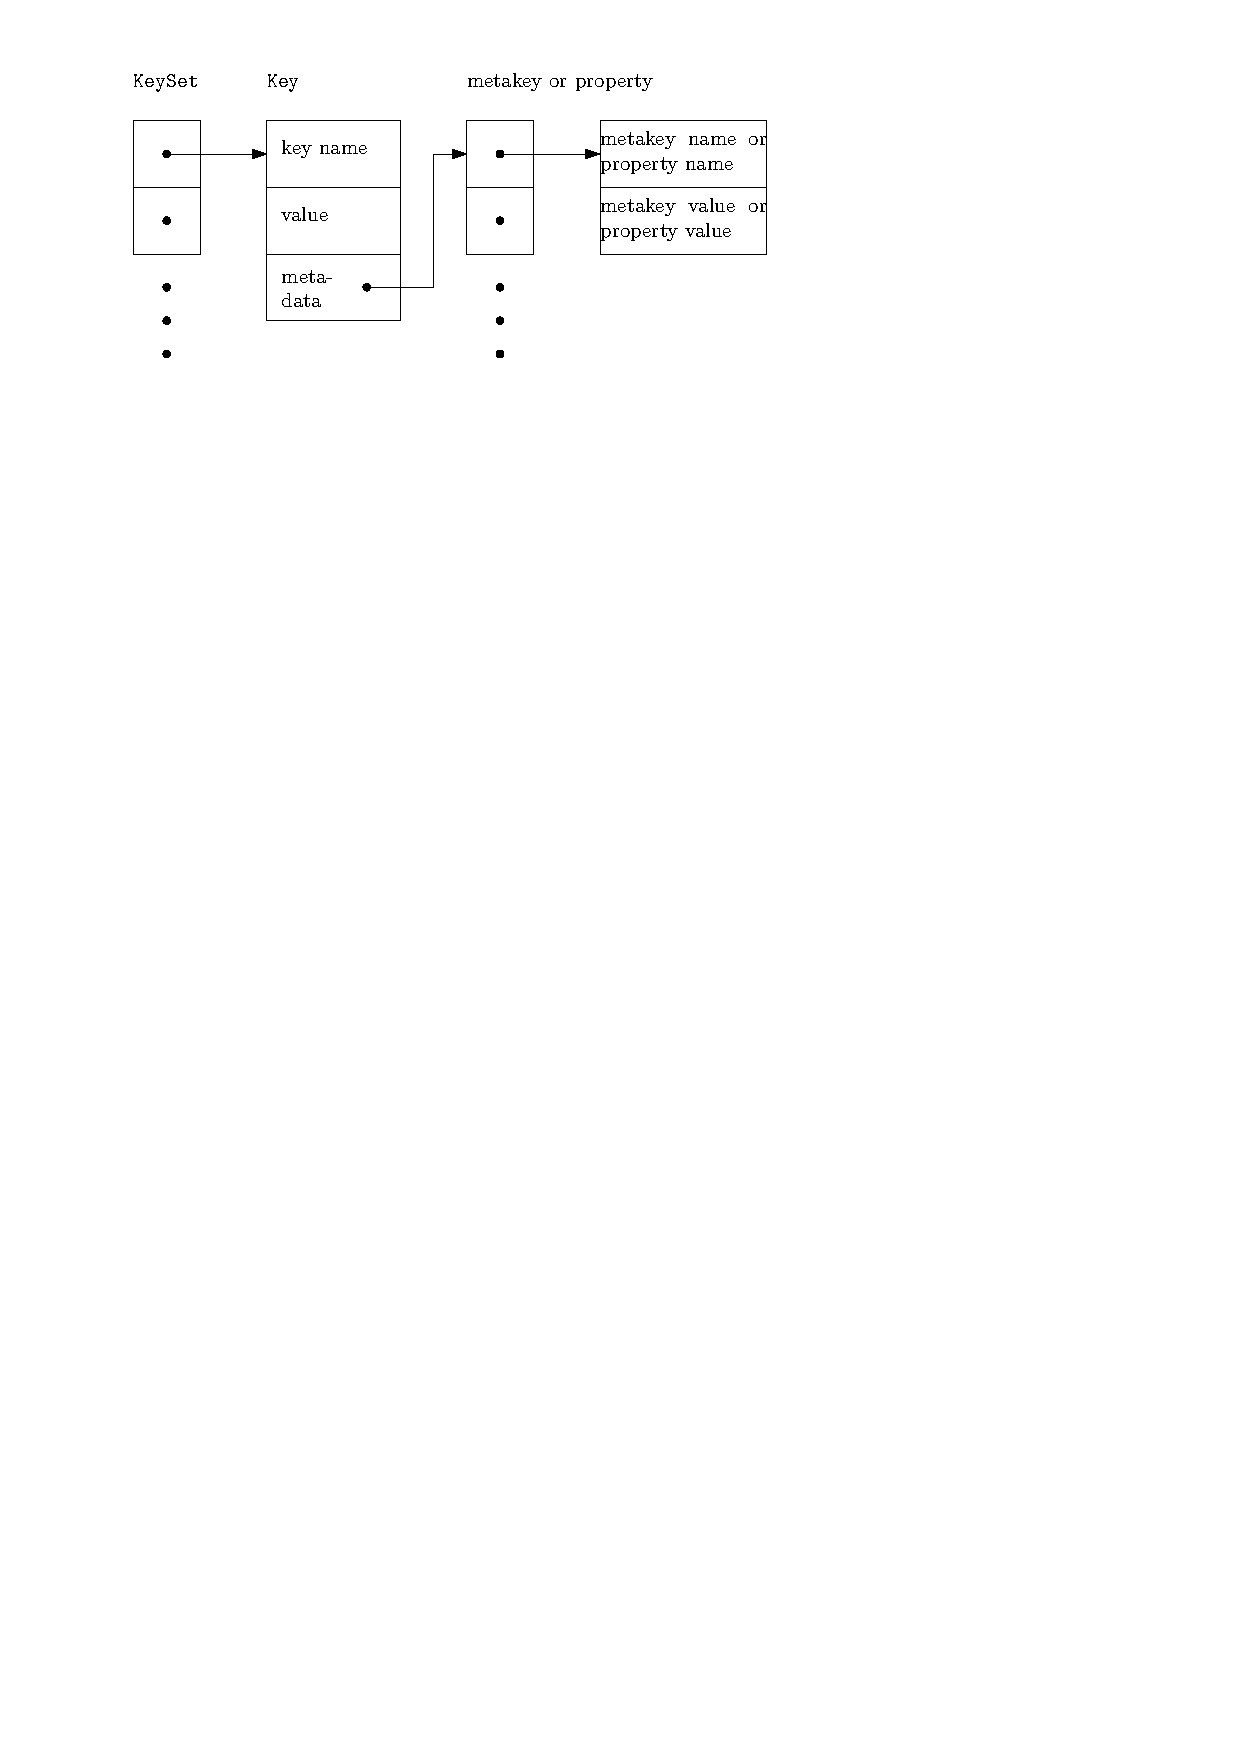
\includegraphics{keyset}
\end{frame}

\begin{frame}
	\frametitle{Recapitulation}

	\methodQuestion{} \question{Which configuration systems/libraries/APIs have you already used or would like to use in one of your FLOSS project(s)?}
	\pause
	\begin{itemize}
	\item command-line arguments (\p{92}, $n=222$)
	\item environment variables (\p{79}, $n=218$)
	\item configuration files (\p{74}, $n=218$))
	\end{itemize}
\end{frame}

\begin{frame}
	\frametitle{Semantics of Command-line Arguments (cont.)}
	\begin{itemize}
	\item passed by main for a new process via \\ (\texttt{int argc, char ** argv})
	\item visible from other processes (e.g., via \texttt{ps aux})
	\item could be passed along to subprocesses but hardly done
	\item need to be parsed by process
	\item portability: differences in parsing
	\item cannot be changed from outside (requires restart, no IPC)
	\end{itemize}
\end{frame}

\begin{frame}
	\frametitle{Talk}
	Miruna Orsa

	Using XML in the day to day work life
\end{frame}



%%%%%%%%%%%%%%%%%%%%%%%%%%%%%%%%%%%%%%%%%% 
\section{Environment Variables}

\begin{assignment}
	\begin{task}
	Brainstorming: What can be part of a configuration specification?
	\end{task}

	\begin{task}
	Advantages/Disadvantages?
	\end{task}

	\begin{task}
	Alternatives?
	\end{task}
\end{assignment}

\begin{frame}
	\methodQuestion{}
	\question{Configuration specification (e.g. XSD/JSON schemas) allows you to describe possible values and their meaning.  Why do/would you specify configuration?}
	\ExecuteMetaData[../book/motivation.tex]{question-introduce-spec}
\end{frame}

\begin{frame}
	\frametitle{Limitations of Schemata designed for Data}
	\begin{itemize}
	\item like XSD/JSON schemas
	\item they are already very helpful but:
	\pause
	\begin{itemize}
	\item not key-value based
	\item not easy to introspect
	\item designed to validate data without semantics: \\ file path vs.\ presence of file
	\item not always possible to extend with plugins
	\item tied to specific formats (e.g. XML/JSON)
	\end{itemize}
	\end{itemize}
\end{frame}

\begin{frame}
	\frametitle{Limitations of Zero-Configuration}
	\begin{itemize}
	\item e.g. gpsd\footnote{\url{www.aosabook.org/en/gpsd.html}}
	\pause
	\item broken hardware or protocols
	\item auto-detection may go wrong
	\item the configuration actually lives elsewhere \\ (e.g., in the GPS devices)
	\end{itemize}
\end{frame}

\subsection{How?}

\begin{frame}
	\frametitle{Types of Specifications}
	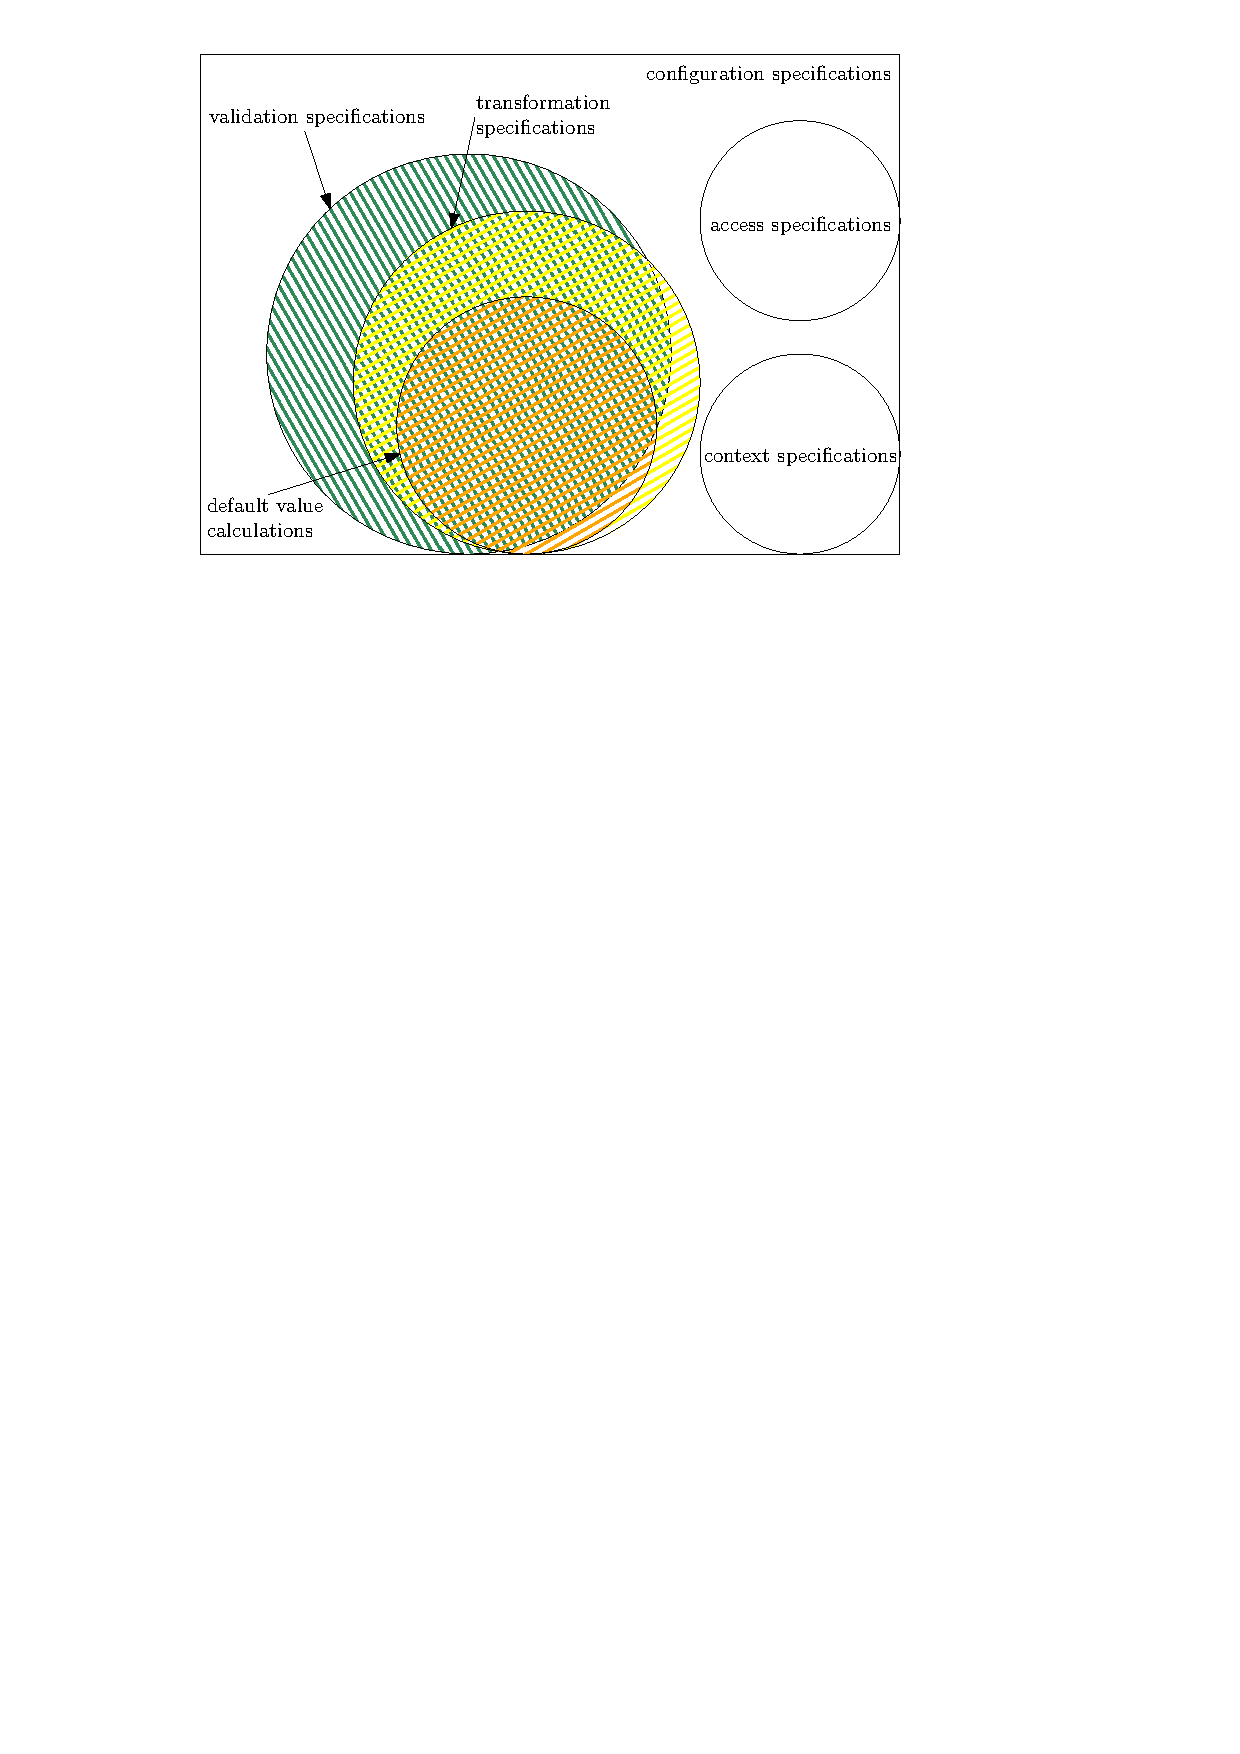
\includegraphics[scale=0.8]{specifications}
\end{frame}

\begin{frame}
	\frametitle{Metalevels}
	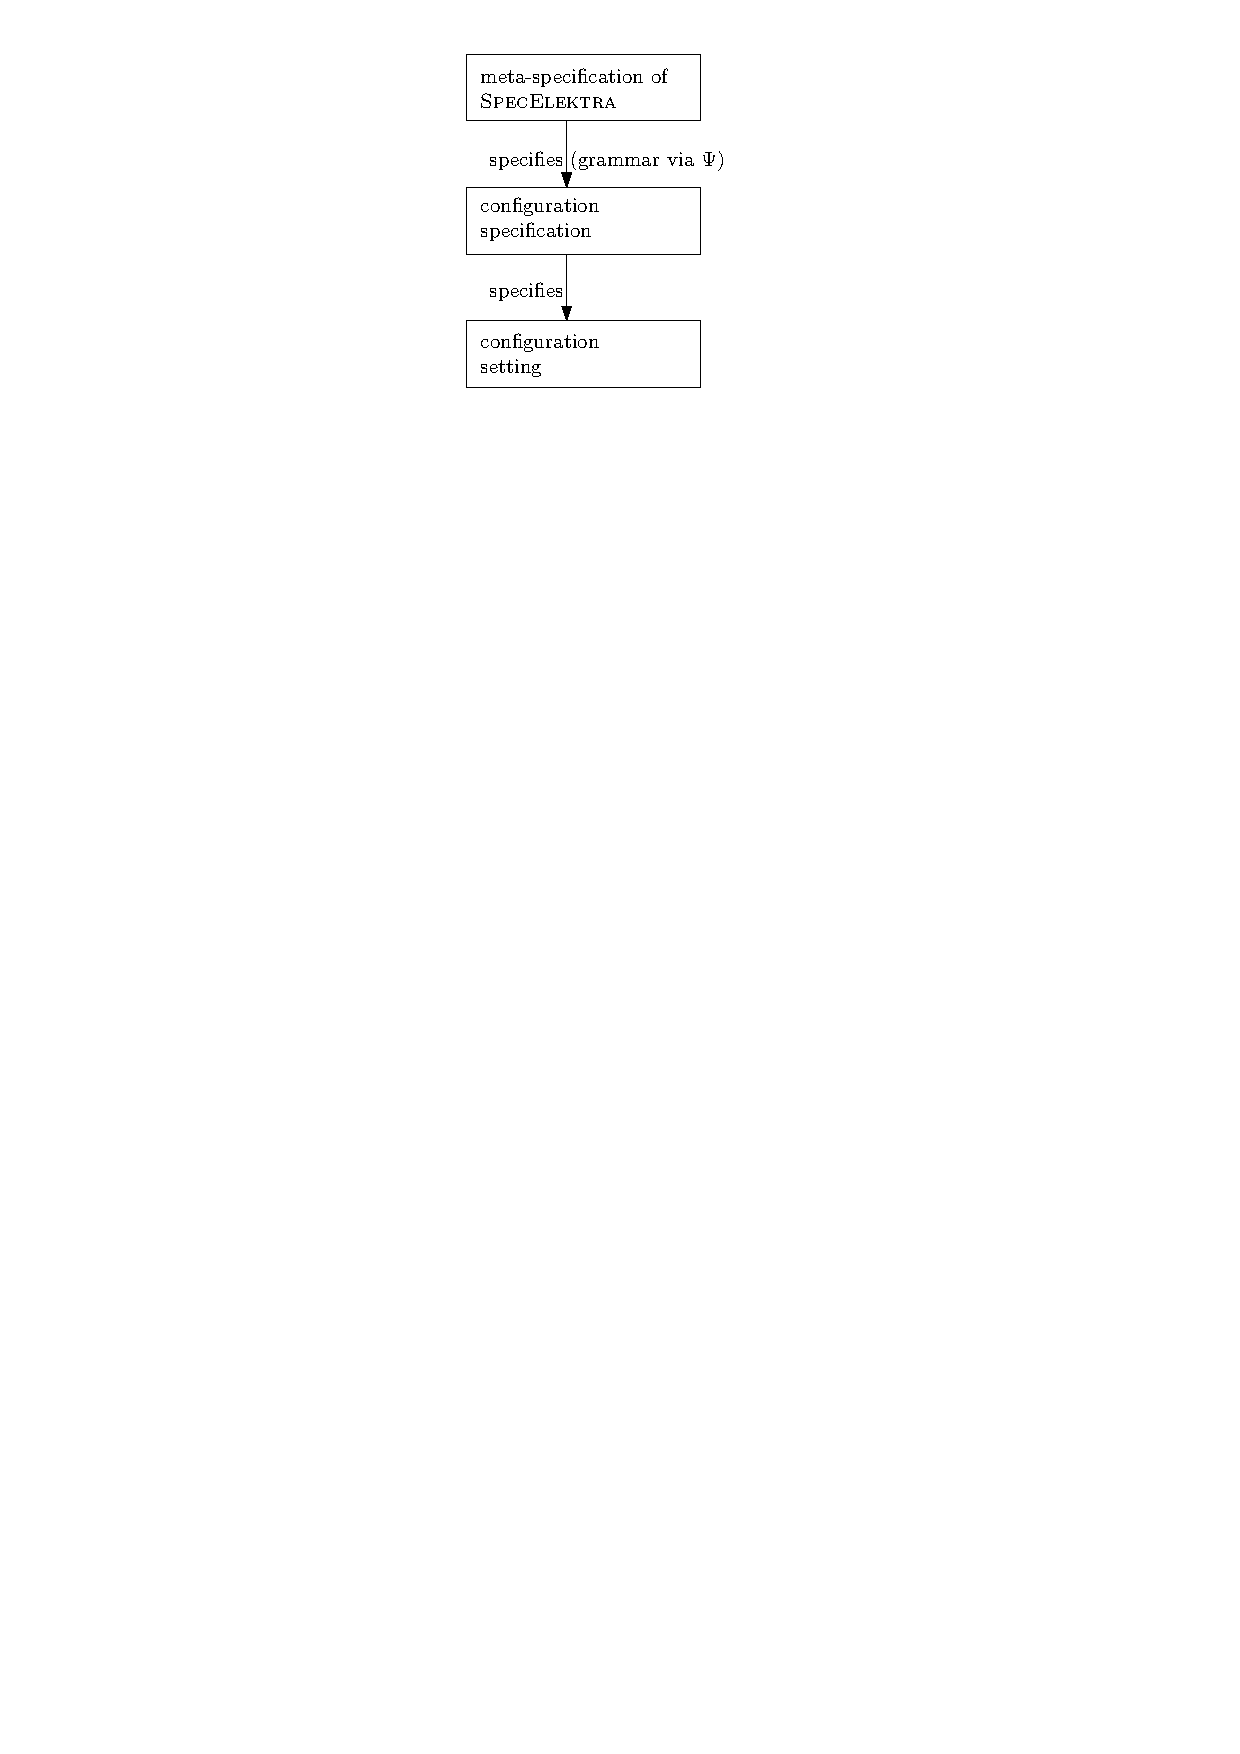
\includegraphics{metalevels}
\end{frame}

\begin{assignment}
	\begin{task}
	What do we mean with a configuration specification?
	\end{task}

	\begin{task}
	Which requirements do we have for a configuration specification?
	\end{task}
\end{assignment}


\begin{frame}
	\frametitle{Requirements}

	\begin{itemize}
	\item formal/informal?
	\item complete?
	\pause
	\item should be extensible
	\item should be external to application
	\item open for introspection (for tooling)
	\item should talk to users
	\item should allow generation of artefacts
	\end{itemize}
\end{frame}


\begin{frame}[fragile]
	\frametitle{Grammar}
	\begin{grammar}
	<configuration specifications> ::= \{ <configuration specification> \}

	<configuration specification> ::= '[' <key> ']' <properties>

	<properties> ::= \{ <property> \}

	<property> ::= <property name> ':=' [ <property value> ]
	\end{grammar}
\end{frame}


\begin{frame}[fragile]
	\frametitle{Example}
	\begin{code}[gobble=4]
	[slapd/threads/listener]
	default:=1
	type:=int
	\end{code}
\end{frame}

\subsection{Examples}

\begin{frame}[fragile]
	\frametitle{Options}

	Environment and command-line options can be considered with:

	\begin{code}[morekeywords={long},gobble=4]]
	[recursive]
	  type:=boolean
	  opt:=r
	  opt/long:=recursive
	  env:=RECURSIVE
	  default:=0
	\end{code}
\end{frame}

\begin{frame}
	\frametitle{Visibility}
	\begin{itemize}
	\item idea: show only relevant settings for specific user group
	\item or disallow editing: accessibility
	\pause
	\item requires user-feedback loops~\cite{xu2015hey}
	\item most-used settings should be best visible (or even enforce them to be changed: against harmful defaults)
	\item think of your users (administrators), \\ only expose what users need
	\item write an rationale why someone needs it
	\end{itemize}
\end{frame}

\begin{frame}[fragile]
	\frametitle{Example}
	\begin{code}[gobble=4]
	[slapd/threads/listener]
	visibility:=developer

	[slapd/access/#]
	visibility:=user
	\end{code}
\end{frame}


\begin{assignment}
	\begin{task}
	Brainstorming: Now, how do we implement such a specification?
	\end{task}
\end{assignment}

\begin{frame}
	\frametitle{Implementations}
	For example:
	\begin{itemize}
	\item generate examples/documentation
	\item auto-completion/syntax highlighting/IDE support
	\item tooling (GUI, Web UI)
	\item validate configuration files
	\item visudo-like
	\item plugins in configuration framework
	\end{itemize}
\end{frame}

\subsection{Calculate Default Values}

\begin{frame}
	\begin{itemize}
	\item idea: make default value better
	\item is the generalization of sharing configuration values
	\item can be combined with visibility
	\pause
	\item can be derived from other configuration settings
	\item can be derived from context~\cite{raab2017introducing}
	\item can be derived from hardware/system (problem with dependences)
	\pause
	\item XServer vs.\ gpsd
	\end{itemize}
\end{frame}

\begin{frame}[fragile]
	\frametitle{Examples}
	Sharing:
	\begin{code}[gobble=4]
	[slapd/threads/listener]
	fallback/#0:=slapd/threads
	\end{code}

	\vspace{1cm}
	Percentages
	\\ (e.g., configured image should be additionally cropped):
	\pause
	\begin{code}[gobble=4]
	[image/width]
	type:=int

	[crop]
	type:=int
	check/range:=0-100
	\end{code}
\end{frame}

\begin{frame}[fragile]
	\frametitle{Examples}
	Context:
	\begin{code}[gobble=4]
	[slapd/threads/listener]
	context:=/slapd/threads/%cpu%/listener
	\end{code}

	\vspace{1cm}
	Calculation with Context
	\\ (e.g., switch off GPS if battery low):
	\pause
	\begin{code}[gobble=4]
	[gps/status]
	assign:=(battery > 'low') ? ('on') : ('off')
	\end{code}
\end{frame}



%%%%%%%%%%%%%%%%%%%%%%%%%%%%%%%%%%%%%%%%%% 
\section{Architectural Decisions}

\begin{frame}
	\frametitle{Software Architecture}
	\begin{itemize}
	\item architecture is high-level description of the overall system
	\item use ready-made patterns and templates for architecture
	\pause
	\item e.g., \url{http://arc42.org/}
	\item architectural decisions~\cite{zdun2007patterns} essential (e.g., Chapter~9 in arc42)
	\end{itemize}
\end{frame}

\begin{frame}
	\frametitle{Architectural Decisions}
	\begin{itemize}
	\item describe decisions that lead to the architecture
	\item open decisions are high-level configuration
	\item useful to have patterns~\cite{zdun2007patterns} and templates, too
	\item template: problem, constraints, assumptions, considered alternatives, decision, rationale, implications, related, notes
	\end{itemize}
\end{frame}

\begin{frame}
	Why are configuration settings added? \\[1cm]
	\pause
	The typical reasons are:
	\ExecuteMetaData[../book/implications.tex]{reasons-adding}
\end{frame}

\begin{frame}[fragile]
	\frametitle{in Configuration Specification}
	\begin{code}[gobble=4]
	[slapd/threads/listener]
	description:=adjust to use more threads
	rationale:=needed for many-core systems
	requirement:=1234
	visibility:=developer
	\end{code}
\end{frame}

\begin{frame}
	\frametitle{Conclusion}
	\begin{itemize}
	\item alarming trend in number and complexity of configuration settings
	\item sharing, visibility and default value calculation often helps
	\item needs abstraction: configuration specification
	\item but also more courageous decisions and periodical reevaluation
	\item different ways to reduce configuration space
	\end{itemize}
\end{frame}


%%%%%%%%%%%%%%%%%%%%%%%%%%%%%%%%%%%%%%%%%% 
\nocite{raab2017introducing}

\appendix

\begin{frame}[allowframebreaks]
	\bibliographystyle{plainnat}
	\bibliography{../shared/elektra.bib}
\end{frame}

\end{document}


